\chapter{Axisymmetric coating process}

\modinfo{Director}{CoatingProcess}
\modinfo{Solvers}{\Idx{FlowSolve}, \Idx{FreeSurfaceReduced}}
\modinfo{Tools}{\Idx{ElmerGrid}, editor}
\modinfo{Dimensions}{2D, Steady-state}

\subsection*{Case definition}

The optical fibers are quite fragile and must therefore be coated with
a layer of polymer before they are stored.  This means that the
coating process must be done with the same speed as the drawing of
optical fibers.  When the diameter of the fiber is only 125 $\mu$m
this sets high demands for the coating geometry since it must provide
even coating at high draw speeds. In Elmer a tailored free surface
boundary condition allows an efficient solution of this particular
problem.


\subsection*{Solution procedure}

The mesh is done with ElmerGrid in the directory coat by the command
%
\ttbegin
ElmerGrid 1 2 coat.grd
\ttend

Therefore the header reads 
\ttbegin
Header
  Mesh DB "." "coat"
End
\ttend
%
The geometry is axisymmetric and the problem is solved in steady state. Typically around 10
iterations is needed to solve the problem but to be on the safe side 30 is set as the maximum.
\ttbegin
Simulation
  Coordinate System = Axi Symmetric
  Simulation Type = Steady State
  Steady State Max Iterations = 30
  Output Intervals = 1
  Output File = "coat.result"
  Post File = "coat.vtu"
End
\ttend
%
In this case there is only one body which comprises of the polymer 
floating between the coating cup and the optical fiber.
\ttbegin
Body 1
  Equation = 1
  Material = 1
End
\ttend

The presented solution used four different solvers. 
The Navier-Stokes solver is required to solve the flow field
for the polymer.
\ttbegin
Solver 1
  Equation = Navier-Stokes
  Stabilize = True
  Internal Move Boundary = Logical False
  Nonlinear System Max Iterations = 5
  Nonlinear System Convergence Tolerance = 1.0e-7
  Nonlinear System Newton After Iterations = 2
  Nonlinear System Newton After Tolerance = 1.0e-2
  Nonlinear System Relaxation Factor = 0.7
  Linear System Solver = Iterative
  Linear System Iterative Method = BiCGStab 
  Linear System Preconditioning = ILU1
  Linear System Max Iterations = 100
  Linear System Convergence Tolerance = 1.0e-10
  Steady State Convergence Tolerance = 1.0e-7
End
\ttend
%
A tailored free surface solver is used to find the 
position of the free surface with a given flow field.
The variable being solved is the displacement of the free surface.
Relaxation is used to avoid over-shooting during the itaration.
This solver does not solve any matrix equations. Instead it solves
the radius from the mass conservation constraint for each node on the
free surface separately. There is a possibility to do the mapping also 
within the solver using a 1D scheme but this is disabled by setting
the \texttt{Perform Mapping} to be \texttt{False}.
\ttbegin
Solver 2
  Equation = "Free Surface Reduced"
  Procedure = "FreeSurfaceReduced" "FreeSurfaceReduced"
  Variable = Dx
  Variable DOFs = 1
  Nonlinear System Relaxation Factor = 0.7
  Nonlinear System Convergence Tolerance = 1.0e-3
  Steady State Convergence Tolerance = 1.0e-3
  Perform Mapping = Logical False
End
\ttend
%
The mesh update solver is required to map the computational mesh
so that it corresponds to the altered geometry.
Here the displacements of the free surface have already been computed
and this solver solves the displacements inside the domain.
Note that solvers 1, 2 and 3 are coupled and therefore the system must be solved iteratively
\ttbegin
Solver 3
  Equation = Mesh Update
  Linear System Solver = Iterative 
  Linear System Iterative Method = BiCGSTAB
  Linear System Preconditioning = ILU
  Linear System Convergence Tolerance = 1.0e-12
  Linear System Max Iterations = 200
  Linear System Symmetric = True
  Steady State Convergence Tolerance = 1.0e-4
End
\ttend
%
In the end, an additional solver is used to compute the forces
acting on the fiber. This does not affect the results.
\ttbegin
Solver 4 
  Equation = Fluidic Force
  Procedure = "FluidicForce" "ForceCompute"
  Calculate Viscous Force = Logical True
End
\ttend
%
Addiationally there are two solvers for saving the results in a form
that is more useful than plain pictures. The \texttt{SaveScalars} saves
the scalar values, such as the diameter and force values,
and the \texttt{SaveLine} saves the free surface.
\ttbegin
Solver 5
  Equation = SaveScalars
  Procedure = "SaveData" "SaveScalars"
  Filename = "scalars.dat"
End 

Solver 6
  Equation = SaveLine
  Procedure = "SaveData" "SaveLine"
  Filename = "kurvi.dat"
End
\ttend
%
The equation includes only the solvers that need a permutation vector 
pointing out the active nodes. Therefore the save utilities do not need to belong
to the set of active solvers.
\ttbegin
Equation 1
  Active Solvers(4) = 1 2 3 4
End
\ttend
%
The material parameters are those of the polymer. Additionally elasticity 
parameters are needed because the solver that updates the mesh is actually
a linear elasticity solver.
\ttbegin
Material 1
  Density = 1.0
  Viscosity = 1.0
  Poisson Ratio = 0.3
  Youngs Modulus = 1.0
End
\ttend

Five different boundary conditions are needed.
The origin is a symmetry axis and thefore the radial velocity is 
set to zero. The axial velovity is the draw velocity.
\ttbegin
Boundary Condition 1
  Name = "Symmetry"
  Target Boundaries = 1
  Velocity 2 = -10.0     ! The draw velocity
  Velocity 1 = 0.0
  Compute Fluidic Force = Logical True
  Mesh Update 1 = 0.0
End
\ttend
%
The free surface has a condition stating that the reduced order free 
surface solver should be solved for that. Additionally the 
free surface is a boundary condition for the mesh update,
and a line to be saved.
\ttbegin
Boundary Condition 2
  Name = "Free"
  Target Boundaries = 2
  Mesh Update 1 = Equals Dx
  Mesh Update 2 = 0.0
  Free Surface Reduced = Logical True
  Save Line = Logical True
End
\ttend
%
At the outlet the radial velocity should vanish and the axial coordinate should
be fixed.
\ttbegin
Boundary Condition 3
  Name = "Outlet"
  Target Boundaries = 3
  Velocity 1 = 0.0
  Mesh Update 2 = 0.0
End
\ttend
%
At the inlet it is assumed that there is no radial velocity and that 
the pressure acting on the surface is zero.
\ttbegin
Boundary Condition 4
  Name = "Inlet"
  Target Boundaries = 4
  Velocity 1 = 0.0
  Pressure = 0.0
  Mesh Update 2 = 0.0
End
\ttend
%
Finally, no-slip conditions are set for the boundaries with the walls of the
coater.
\ttbegin
Boundary Condition 5
  Name = "No-slip"
  Target Boundaries = 5
  Velocity 1 = 0.0
  Velocity 2 = 0.0
  Mesh Update 1 = 0.0
  Mesh Update 2 = 0.0
End
\ttend


\subsection*{Results}

\begin{figure}[tbhp]
\begin{center}
  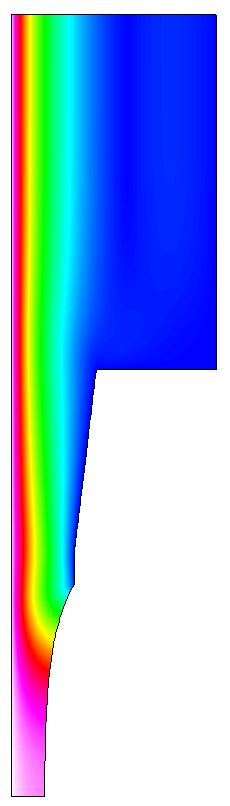
\includegraphics[height=0.6\textwidth,angle=0]{coat_vel}
  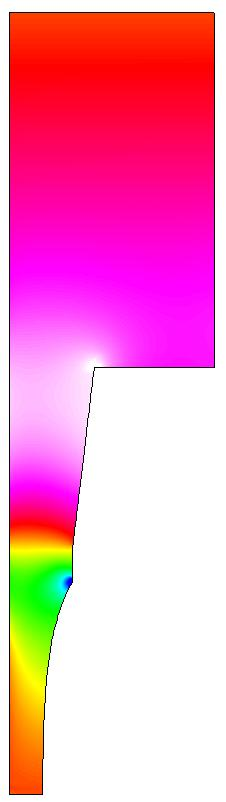
\includegraphics[height=0.6\textwidth,angle=0]{coat_pres}
  \caption{The velocity and pressure fields in a simple coating geometry.
	The solution utilizes the reduced dimensional free surface solver.}
\end{center}
\end{figure}

In the given case solution is obtained after 13 iterations.
The solution gives the final radius, the forces, and the profile of the 
free surface. To visualize the true free surface you may visualize the
last timestep using Paraview, or some other software capable of reading
VTU files. 
%ead in the only the last timestep and in \texttt{ElmerPost} give the following
%ommands:
%ttbegin
%ath nodes0 = nodes
%ath nodes = nodes0 + Mesh.Update
%ttend
%ote that this does not work if there is more than one set of variable values.


\vfill
\mbox{}
